\documentclass[../physical_computing.tex]{subfiles}

\begin{document}

\newcommand{\crlf}{\symbol{92}n\symbol{92}r}
\newcommand{\linefeed}{\symbol{92}n}

\chapter{Lab Exercise 7 - Embedded Processor Cores}
\label{sec:appendix_7}

In this exercise we will install a microblaze soft processor core on the BASYS3 board, then program the core in the 'C' language that we
started to learn in the last seminar. 

\section{Hardware installation}
\label{sec:hardware}

First, the hardware. Start Vivado as usual, and select 'Create project'. Everything follows as it did
for previous exercises at the start. Skip adding any source or constraint file. When you get to the 'Default part' page, you will notice that
near the top of the window there are two tabs, labelled 'Parts' and 'Boards'. The 'Parts' one is lit up by default. You need to instead select
the 'Boards' tab. When you do this, you should be able to scroll down and highlight 'Basys3', then click next and finish. The project summary
should now look roughly as in Figure \ref{fig:project1_summary}, up to the paths to things, which will be different for you.

\begin{figure}[h!]
    \centering
    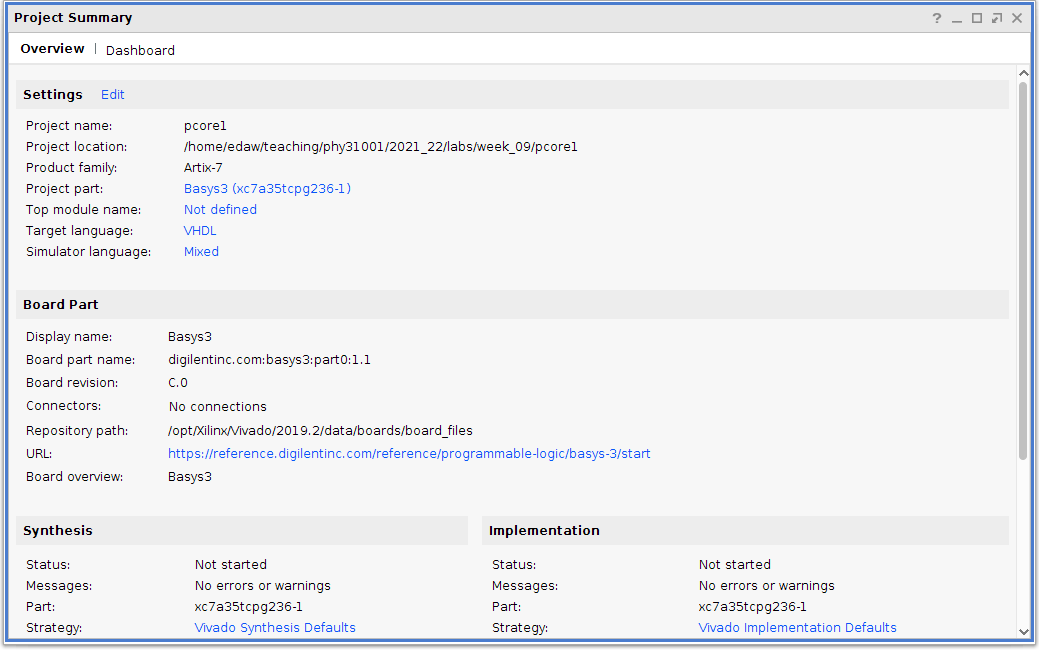
\includegraphics[width=0.8\textwidth]{figures/project1_summary.png}
    \caption{The project summary after setting up for use with the Basys3 board.}
    \label{fig:project1_summary}
\end{figure}

Next select 'Create Block Design' and accept the default name (project\_1). In the empty diagram press the button to add IP, and in the 
menu that appears search for MicroBlaze. You want the one at the top that is just MicroBlaze on its own. Double click on it and it shows
up in your window. Next, you'll need a UART interface, so you can connect your laptop to the processor to either make input or see output.
So, click on the '+' button at the top of the design window. The same menu appears again. This time, you do a search for UART. This stands
for 'Universal Asynchronous Receiver Transmitter' - it's a protocol for two devices talking to each other where there is no handshaking, ie,
both devices can send at any time no matter what the other device is doing. You want AXI Uartlite. Double click on this and it will also
appear in your block diagram.

You will need one other piece. This is the 'system clock'. This is board dependent, because the clock is supplied by an external crystal,
which in the case of the BASYS3 board is a MEMs device that produces a single ended output, meaning that the clock signal is just a square
wave on a single wire. The board tools in Vivado assume a professional-grade differential clock signal, so you need to defeat the tendency 
of the connection automation tools to make everything differential. TO do this, go to the 'Board' tab under where it says BLOCK DESIGN
(other tabs are sources, design, signals...). In the board tab you'll see features of the board rather than the FPGA. Drag the top one 
labelled System Clock onto the block diagram.

At this point you have three pieces of hardware but no idea how to connect them together, or indeed how to custommise them where necessary.
For the first 'Hello World' project, you probably don't need to change anything. However, the default amount of memory assigned to the 
processor core is tiny, so I'd like you to increase this. Highlight the microblaze core (it turns orange), and click on the blue link 
above it in the window labelled 'Run Block Automation'. In the window that appears, change the local memory from {\rm 8\,kB} to {\rm 128\,kB}.
Now your programs are unlikely to run out of memory when deployed to the core. Change nothing else and click 'OK'. This will induce the
appearance of several more blocks in the design, a 'Clocking wizard', a unit called 'Processor System Reset', a debug module, and
some 'Microblaze local memory'. Your diagram should now look something like that in Figure \ref{fig:afterblockautomation}

\begin{figure}[h!]
    \centering
    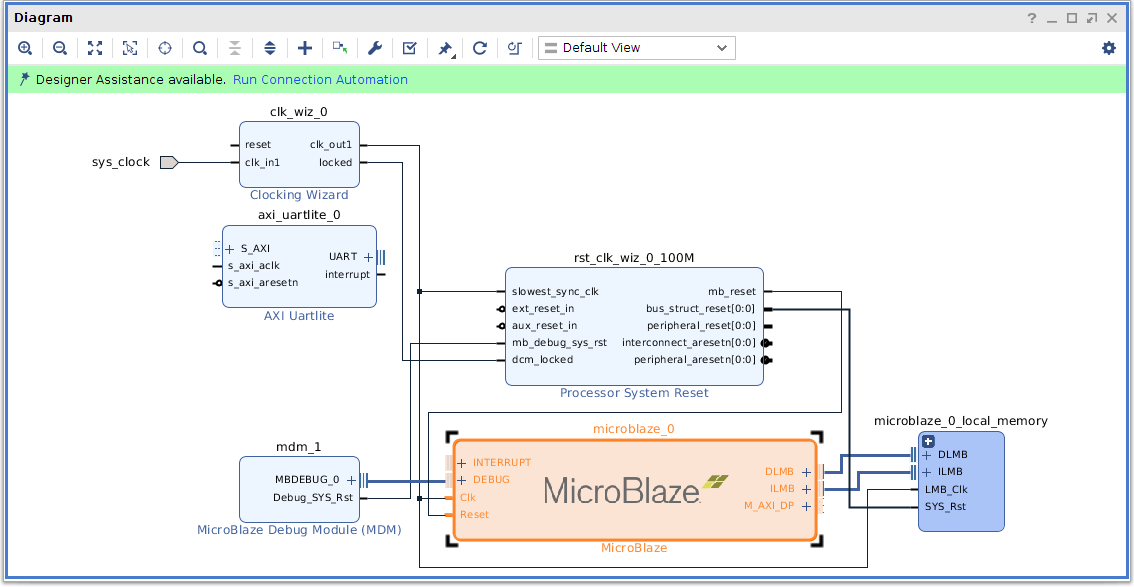
\includegraphics[width=0.8\textwidth]{figures/afterblockautomation.png}
    \caption{The block design after block automation, but before connection automation.}
    \label{fig:afterblockautomation}
\end{figure}

You'll now notice that there are some remaining unconnected subsystems. Most significantly, there are no connections to the clock on the 
board or the USB uart (serial port) output. However, the remaining link at the top of the window, called 'Run Connection Automation' can
take care of this. This is because the board support package for Basys3 contains much information about non-FPGA components on the board, 
so that using this support package, Vivado can ensure that the various components needed to support the microblaze core are found
and connected up correctly. Click on the `Run Connection Automation' link and check the `All Automation' box, to connect everything together.
More wires and blocks should appear. A notable one is the AXI Interconnect. AXI is the bus that is used as a general purpose connecter to peripherals, in 
the same way as the PCI and PCI express buses are used to connect memory, graphics cards, network cards, etc, to the microprocessor inside 
a PC. It is needed here to connect the UART controller to the Microblaze processor core.

There are a couple of final steps before we are done with this diagram. First, check that everything that needs to be connected, is connected.
A rudimentary diagram checker is built in to Vivado - it's the box with a tick mark in it above the diagrm window. Click on this, and you should
see a window appear where it says 'Validation succesful....'. Click 'OK'. If you don't  see this, then check you have carried out all the 
steps described above. There is also a tool for tidying up your block diagram so that it looks less like a plate of spaghetti. This is
the small arrow going around in a circle icon that is above the block design. Click this and nothing changes with the wiring, but things
are moved around so that they look a lot tidier. See Figure \ref{fig:afterconnectionautomation}. You'll notice that some more extra
modules have appeared. 

\begin{figure}[h!]
    \centering
    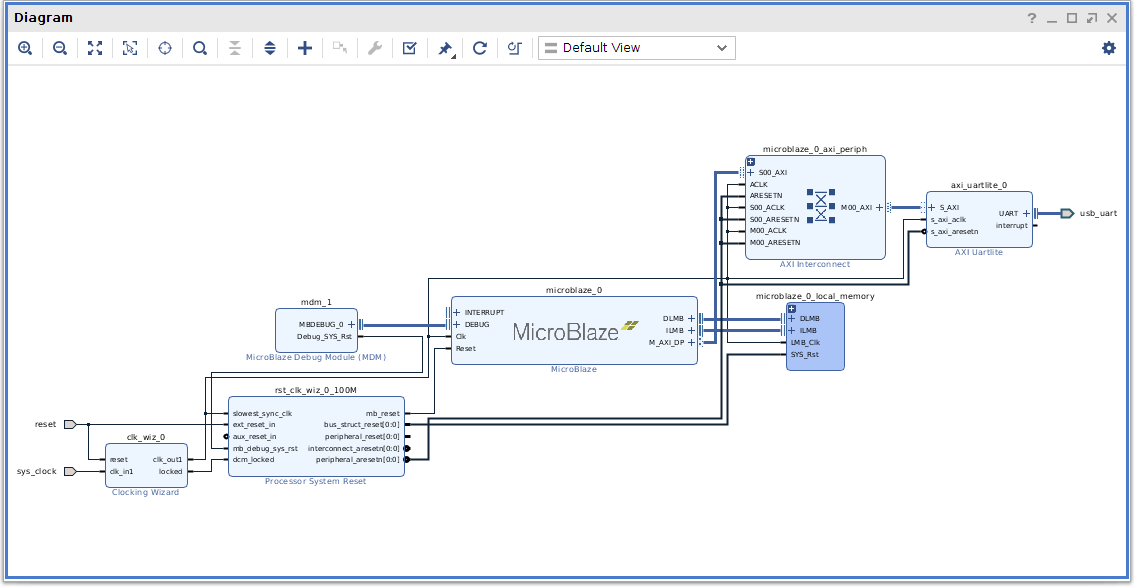
\includegraphics[width=\textwidth]{figures/afterconnectionautomation.png}
    \caption{The block diagram after connection automation has been run.}
    \label{fig:afterconnectionautomation}
\end{figure}

One more thing that is worth looking at. The AXI bus is more complicated than the simple parallel and/or serial buses with which you
are already familiar. It's an example of a memory mapped bus. This is needed when there is the potential for more than two devices
to be connected together by a bus. The obvious potential for data to end up arriving at the wrong device is guarded against by
associating a memory map with the bus. Each device on the bus occupies a pre-determined set of addresses in this memory map, so that
if you want to communicate with a particular device, you just read from, and/or write to, addresses associated with it. If you 
click on the 'Address Editor' tab above the diagram, you'll see that there are 32 bit address buses associated with data and 
instructions for each of the memory controllers and the UART device. This is shown in Figure \ref{fig:memorymap}.

\begin{figure}[h!]
    \centering
    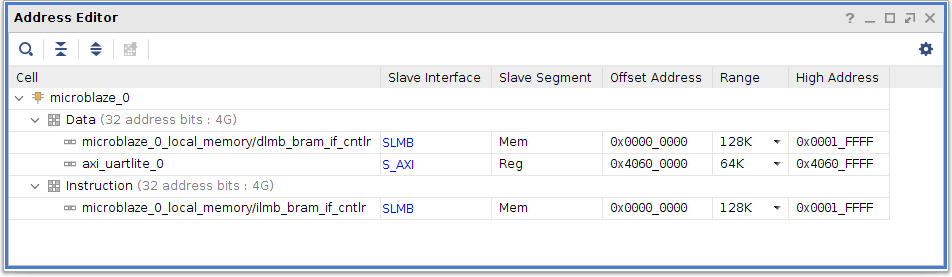
\includegraphics[width=0.8\textwidth]{figures/memorymap.png}
    \caption{Address space of our soft core hardware}
    \label{fig:memorymap}
\end{figure}

If you wanted to, you could edit both the Offset address, 
which is the address where the memory mapped to the device starts (sometimes called the base address of the device), and also 
the size of the space it occupies. In this case, we want to leave it alone! Needless to say when we come to adding shared memory,
this will have a base address on the bus too, which we will need to know to write programs that use this shared memory.
Save the block design by using 'Save block design' under the File menu at the top left of the Vivado window.

\section{Hardware build}
\label{sec:hardwarebuild}

So far we have been laying out the hardware to support the soft core. Now we need to build it. Under the hood, all of the blocks 
that we have been dealing with are in fact VHDL modules connected together with port map syntax. The compilation is of the VHDL, 
not of the graphics. Consequently, like every VHDL project, we need a top level VHDL program which contains the port map statements
that actually connect everything together. There will also be some numerical inputs added, specifying, for example, the memory
size for the MicroBlaze core, and anything else in the set of components that we have added which is in need of customisation.
To create this file, go to the pane directly under where it says BLOCK DESIGN - design\_1. One of the tabs reads Sources. Click on
this tab to select it. Under 'Design Sources (1)', you should see an entry for design\_1. Right-click on this and in the ensuing 
window select 'Create HDL Wrapper...'. Select the default of allowing Vivado  to manage wrapper and auto-update; this means that if
you make changes to the diagram, those changes will automatically result in corresponding modifications to the wrapper. Click
'OK'. After a short pause, the hierachy under Design Sources should have a top level object called design\_1\_wrapper. This is
actually a VHDL file. You don't need to know what is in it, but double-click on it if you are interested. Your diagram is still behind
the code that appears, it's just in a tab called Diagram.

From now on, hardware wise, it's back to how we are uesd to doing things. Click on 'Run Synthesis'. Make sure you enable all 4 
cores on your machine for synthesis as this time Vivado has to build all the components in your diagram, including the soft core
processor, and this will take some time. If you click on the 'Design Runs' tab in the bottom window and expand all the items in 
the list, you'll get progress bars for each of the sub-builds as they occur. You should see more than one object being built
at the same time. The view in this window with everything expanded is shown in Figure \ref{fig:designruns}

\begin{figure}[h!]
    \centering
    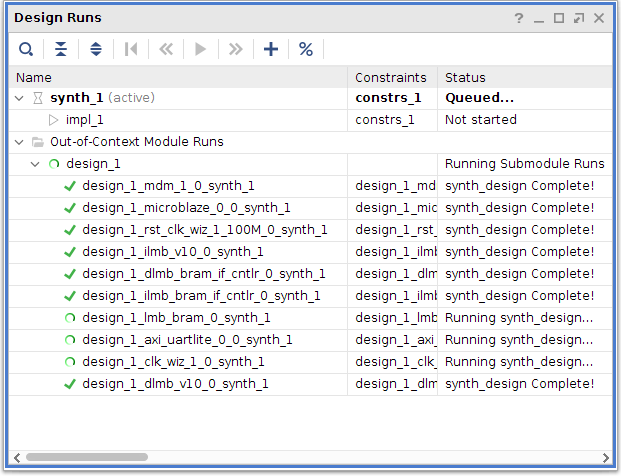
\includegraphics[width=0.8\textwidth]{figures/designruns.png}
    \caption{The Design Runs tab during the soft machine build. Notice that three blocks are being built at once, one by each
    of three cores in the CPU. This build is why I bought nice-ish laptops for the course.}
    \label{fig:designruns}
\end{figure}

After synthesis, if all goes well, then you should be able to go ahead and run implementation, then generate bitstream, in the usual
way. When you have generated the bitstream, you will need to click on 'Cancel' because we don't want to open the hardware manager
quite yet.

\section{Exporting your hardware design}
\label{sec:export}

Finally, we need to export the bitstream to the software development kit, where it will be combined with the program to be run on the MicroBlaze core. To do this, in the File menu in Vivado, select 'Export' and then 'Hardware'. In the window that appears, check the box that says `Include bitstream' and hit 'OK'. Notice that the name of the file it produces is
`design\_1\_wrapper.xsa'. This is the file we will need to point to when we launch Vitis, the software development kit where we will produce our 'C' program. Leave Vivado open.

\section{`Hello World' program}
\label{sec:helloworld}

Launch Vitis using the red stylised `V' icon in the left hand toolbar on your laptop. When asked for a workspace directory, browse to the top directory of the project you just created in Vivado. It doesn't have to be there, but it seems sensible to keep everything in the same place. Click 'Launch'. A window should appear with various options. Select 'Create Application Project'. The project name should be (for want of a better idea) hello\_world. Click 'next'. At the top of the window that follows, there is a tab called 'Create a new platform from hardware'. Select this tab, then press the $+$ button in the ensuing screen. Navigate using the file browser to the .xsa file from your hardware project, and then press the 'Select' button in the top right of the screen. This .xsa file should be added to the list of available platforms, and be highlighted. The platform selection screen should resemble Figure \ref{fig:selectplatform}. Click on 'Next'. The next screen has the defaults correct - we are compiling for microblaze\_0 (the only processor core in your hardware - there could in general be more than one), in a standalone operating system (you are building code for the 'bare metal' chip - you don't have an operating system kernal running your code at all), and you are going to develop your application in C. The default application template is, as it always is, a program conveniently called hello world. Click finish on the bottom right.

\begin{figure}[h!]
    \centering
    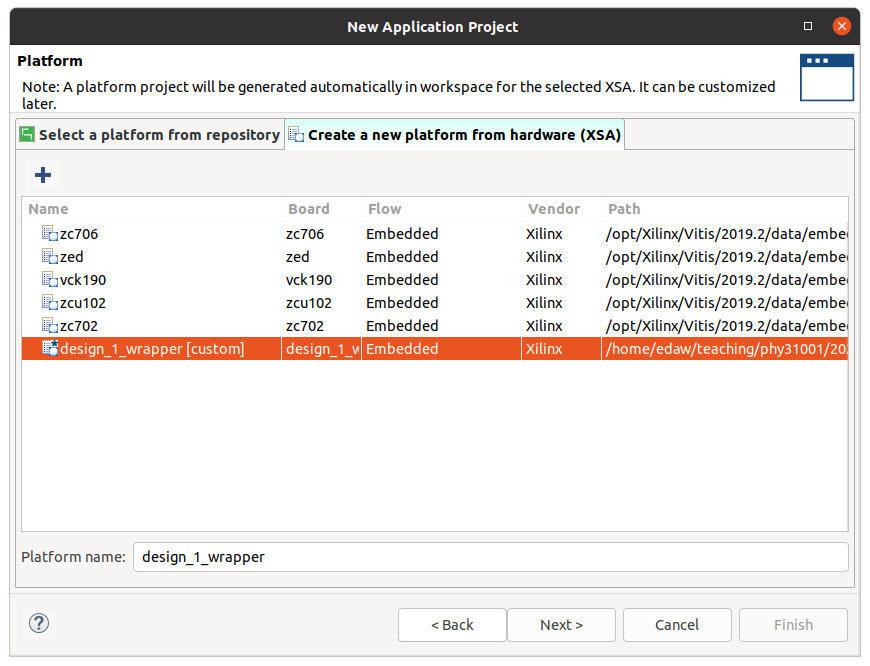
\includegraphics[width=0.8\textwidth]{figures/selectplatform.png}
    \caption{The choice of platforms after your newly created hardware platform is added.}
    \label{fig:selectplatform}
\end{figure}

The main IDE (integrated development environment) window now appears. This is the environment where you will write your code. It appears similar to Figure \ref{fig:firstide}.

\begin{figure}[h!]
    \centering
    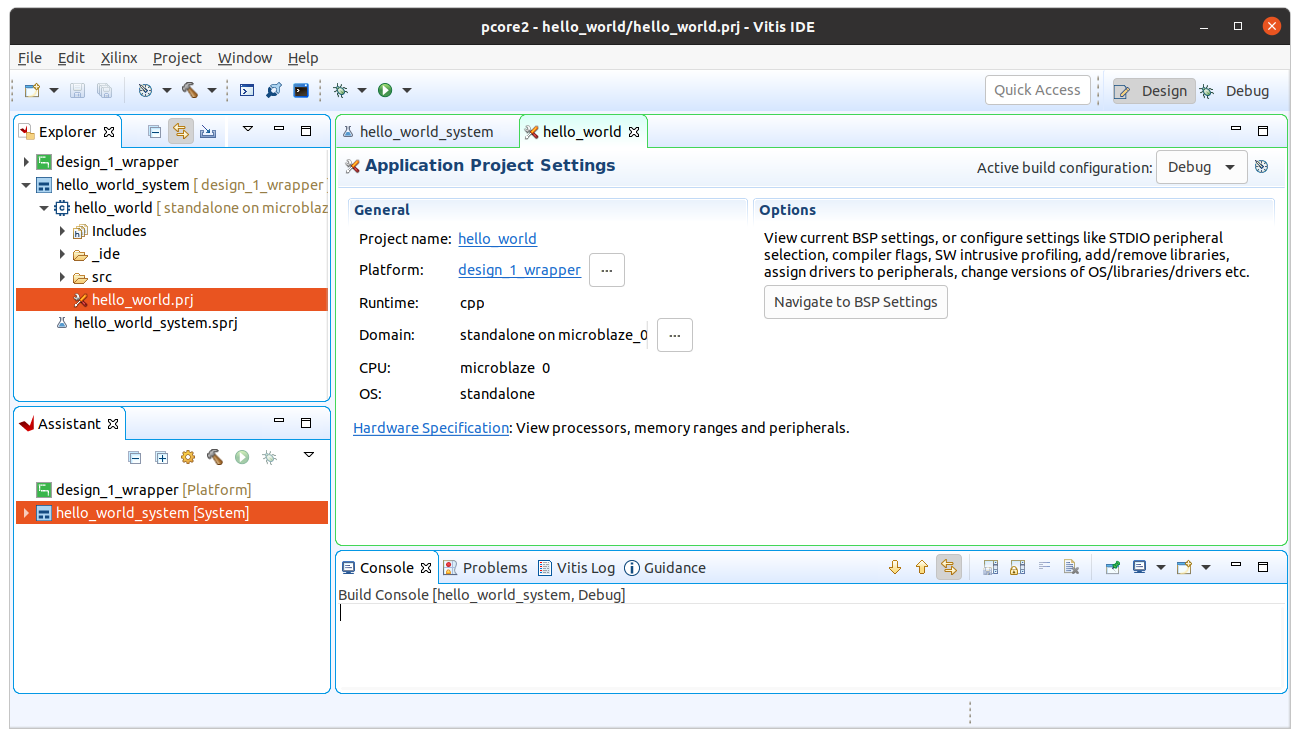
\includegraphics[width=\textwidth]{figures/firstide.png}
    \caption{The IDE when you first enter it for a new system}
    \label{fig:firstide}
\end{figure}

The SDK project uses a standard variety of graphical development
environment known generically as Eclipse. Eclipse graphical interfaces
are ubiquitous in software engineering. The interface is based 
around a file system that looks very like a standard PC directory 
structure. The top level directories are on the left in the Explorer
window. They are design\_1\_wrapper, which contains code relevent to 
the hardware. For now we'll leave that one shut. Then there is the 
folder hello\_world\_system, which contains everything having to do with the
code we are about to develop for the board. Each folder contains an
arrow that you can click on to reveal the folder contents, which may
be source files or sub-folders or both. Open the hello\_world\_system
folder, and you will see a subfolder called hello\_world. Open this
subfolder, and you will see several sub-sub-folders. One of them is
called src (as usual short for source code), so open that one. In
this folder you will see a file called helloworld.c . This contains the
source code that will allow the processor core in your hardware system
to greet you. Double click on helloworld.c to open it and view its 
contents.

The first 46 lines are an extended comment that contains things like
the name of the developer, when it was written, a contact email, and
a summary of what the code does. It's a good idea to get into the habit
of providing this information, especially if you think you might one
day develop software in a team. Lines 48 to 61 contain the actual code,
reproduced below.

\begin{minted}{c}
#include <stdio.h>
#include "platform.h"
#include "xil_printf.h"

int main()
{
    init_platform();

    print("Hello World\n\r");

    cleanup_platform();
    return 0;
}
\end{minted}

The three include statements cause the preprocessor to reproduce the
contents of those files at the top of the code before compilation. They
typically contain further preprocessor commands, which are in turn 
executed, and function declarations as discussed in class. For 
example, a function print() is used in the code - the declaration of
print() will be in one of the headers. Note that print() is NOT a 
commonly used C function - this is one that xilinx have added 
themselves. The more common C print command is printf. Xilinx have 
written their own printf(), which is a more sophisticated print command,
and it is declared in xil\_printf.h. We will use it in a while.

It is pretty straightforward to see by eye what this function does.
The init\_platform() and cleanup\_platform() statements are doing some
special functions that must be required by microblaze. We don't need
to know what they do right now, but we could if we wanted to go and
read the source for these functions to find out. The only line which 
we need to know about for now is the print line, which is obviously 
going to attempt to print something. Just so we know that we are 
not cheating, edit the file substituting your name for World. After
this edit, use ctrl-s to save the file. 

Now highlight the hello\_world\_system folder, and click on the
hammer icon at the top. This will compile the project, producing 
an executable that can eventually be loaded onto our hardware.
A small pane at the bottom with a tab called Console shows you
the build commands and progress. You can click on the rightmost 
icon in this small pane to maximise the window and see what it
contains. It compiles two C programs, one called helloworld.c
(the one we just examined) and the other called platform.c. The latter
one is probably the 'microkernel' that initialises the processor, 
connects it to the memory where are program is stored, and then
positions the stack pointer that carries out the commands at the 
command corresponding to the start of the main() function. After
these two C programs have been built, then a second code called the
linker joins them together and makes the executable, which is called
hello\_world.elf . This is the program - the 1s and 0s that define
the instructions and data that are fed the microprocessor state
machine.

If the build worked, then you will see at the bottom, in blue,
the time at which the build finished, and how long the build took
in milliseconds. This was measured using the clock built in to 
your laptop to do the timing. To put this window back into the 
small pane at the bottom, click on the rightmost icon in the 
window again, which should now be two small overlapping rectangles.

Now we are ready to run your first C program. Go back into Vivado,
open the target manager, and programm the Basys3.

Having programmed it, start the application called 'Serial port
terminal' in the left hand tool bar - the icon looks like a 
9 pin d-sub connector (the old standard connector for serial 
cables). Once you have started it, click on the 'Configuration'
pull-down at the top and select port. You need to change the 
Port to /dev/ttyUSB1 and the Baud Rate to 9600. Other than that,
leave everything the same, then click Okay.

Now finally go back to your Vitis project window. Highlight the\\
\mbox{'hello\_world\_system'} folder in the Explorer pane. Now at the top
of the window, find the rightmost icon, which is a green circle
with a white 'go' arrow in it. Press on this button. A progress
bar will appear whilst your hello\_world.elf program is transferred
to the microblaze core. You should then see Hello (your name) appear
in your UART terminal window. You have turned your Artix7 into
a computer and it has run its first program. Well done.

This is a laborious process. It clearly isn't worth it just to have
the computer say hello, but you can imagine that we can now make
our computer do more sophisticated things. For a start, we can 
try out some of the C programming that I introduced in the last
seminar. Then we can perhaps move on to getting the computer to 
interact with programmable logic.

\section{More C Programming}
\label{sec:morecprogramming}

First I'd like you to use the more sophisticated xil\_printf() command
instead of the simple print(). This is because xil\_printf() allows
us to print variables as well as just text. For now however, just 
make the replacement of the print statement with xil\_printf as
follows:

\begin{minted}{c}
xil_printf("Hello World\n\r");
\end{minted}

Press the hammer again to rebuild, then the green arrow to re-run.
You should get another Hello statement. I don't care at this point
if you use World or your name. You may by now be wondering what
the \texttt{\crlf} charcters at the end mean. These are speical non-
printing characters, called 'new line' and 'carriage return'. To
understand why they are needed, you need once to have used an old
fashioned mechanical typewriter. I am sure none of you have. However,
on an old typewriter, in order to type two lines of text, you needed
to type the first line, and then return the carriage that contained
the paper to the beginning of the line, and move a roller that advanced
the paper upwards by one line. There, that's two operations. That old
mechancial reflex-action has ended up finding its way into modern
ascii text files! Furthermore, whether you need \texttt{\crlf} or
just \texttt{\linefeed} is believe it or not system dependent! On Linux
machines you just need \texttt{\linefeed} and on microblaze processors you
need \texttt{\crlf}. It's a mad world sometimes.

Next I want you to make some slightly more extensive modifications
to the code, as below. 

\begin{minted}{c}
int main()
{
    /* declare a 32 bit unsigned integer variable called count */
    u32 count;
    init_platform();

    /* loop over count values between 0  and 9 inclusive */
    for(count=0;count<10;++count) {
    	/* display greeting and current count value */
    	xil_printf("Hello Ed %u\n\r",count);
    }

    cleanup_platform();
    return 0;
}
\end{minted}

I have added some comments next to the new things I have 
inserted to explain what they do. You should put comments in your
code as well. The first addition is the declaration of a variable
called count. This is at the top of the main() function. The
variable is of type u32, which is Xilinx's 32 bit unsigned integer
data type. This variable is used as the counting variable in 
a for loop. The for loop starts with count=0, and cycles whilst
count is any value less than 10, incrementing by 1 at the end of
each iteration. 

Finally, I have altered the xil\_printf statement which is now 
inside the body of the loop. I have included a \%u after Hello
Ed (my name, of course). This is called a format field specifier.
It tells the print function to expect to print an unsigned integer
there. Then, after the end of the double quotes that enclose the 
text and format field specifier, there is a comma, followed by the
name of the variable to be printed.

The xil\_printf() function can take an arbitrary number of arguments,
where each argument is a new variable to be printed. So, for 
example we could write instead the following inside the loop:

\begin{minted}{c}
xil_printf("2 times %u is %u\n\r",count,2*count);
\end{minted}

This time there are two format field specifiers in the xil\_printf(),
and two corresponding variables to be printed. The first is still
just count, and for the second I've built some simple multiplication 
arithmetic into the print statement, so that the effect is to print
out the first 10 elements of the 2 times table (including 2 times 0).
Note that the format field specifier is the same both times, because
both things to be printed are integers.

You can play around more with making the arithmetical operation 
more complicated, but don't push your luck. You will find you can't
do more sophisticated maths than add, subtract, multiply and perhaps
divide. xil\_printf() may also have trouble printing out floating
point numbers. After all, the processor is super-compact and running
on a multi-purpose FPGA, not a special purpose CPU.

Now lets make a conditional statement inside our for loop. Modify 
the loop to the following code:

\begin{minted}{c}
for(count=0;count<10;++count) {
    /* test to see if it's 5, if it is, print yipee 5 */
    if(count==5) {
    	xil_printf("Yipee, count=%u\r\n",count);
    } else {
    	xil_printf("count=%u\r\n",count);
    }
}
\end{minted}

This code will print count=(value) every cycle of the for loop, 
but will print something different when the value is 5. It might
occur to you that you can achieve the same effect with slightly 
simpler syntax, as below.

\begin{minted}{c}
for(count=0;count<10;++count) {
    /* test to see if it's 5, if it is, print yipee 5 */
    if(count==5) {
    	xil_printf("Yipee, ");
    }
    xil_printf("count=%u\r\n",count);
}
\end{minted}

This saves an else statement. It exploits the fact that every 
cycle we are displaying the value of count. The only thing that 
is added is the Yipee, . If we use xil\_printf without the 
\texttt{\crlf} for the yipee, then the next xil\_printf statement
will complete the line of text. 

If you prefer to spell out your numbers with letters, we can
implement a case statement that does this as follows:

\begin{minted}{c}
    for(count=0;count<4;++count) {
    	xil_printf("count is ");
    	/* switch statement to act depending on count */
    	switch(count) {
    	case 0:
    		xil_printf("zero");
    		break;
    	case 1:
    		xil_printf("one");
    		break;
    	case 2:
    		xil_printf("two");
    		break;
    	case 3:
    		xil_printf("three");
    		break;
    	default:
    		xil_printf("out of range");
    	}
    	xil_printf(".\r\n");
    }
\end{minted}

Note that this time I have cut the for loop off above 3, because
I didn't want to write out ten case statements! Case structures
are often a good alternative to multiple if statements, in the case
where there is a large set of possibilities and you want to address
all of them. The break; statement is a bit of an oddity of the 
language. You need one at the end of each case. It is also a good
practice to have a default action if none of the cases are satisfied,
otherwise the behaviour of your code can be ill-defined. Note
also that I include text before and after the case structure so that
in each case I get a complete sentence.

Now that we are getting more complex code, you may find that you 
start to make mistakes. For example, you might miss a semicolon.
When you try to compile this will generate errors. For each error, 
the code editor will put a red 'x' next to the line number where
the problem originated. If you hover above this 'x', a message will 
appear telling you the error message this line resulted in. This 
can be a useful way of figuring out what you did wrong.


\end{document}